\documentclass[10pt,a4paper]{article}
\usepackage[utf8]{inputenc}
\usepackage[T1]{fontenc}
\usepackage[usenames,dvipsnames]{xcolor}
\usepackage{amsmath}
\usepackage{amsfonts}
\usepackage{amssymb}
\usepackage{graphicx}
\usepackage{subcaption}
% Package for si units
\usepackage{siunitx}

% Packages for making pictures with LaTeX
\usepackage{tikz}
\usetikzlibrary{shapes,arrows,positioning,fit,backgrounds,calc}
\usepackage{pgfplots}
\pgfplotsset{compat=1.16}
\usepackage{tikzviolinplots}
\usepgfplotslibrary{external}
\tikzexternalize
\usepackage{minted}
\usemintedstyle{gruvbox-light}
\usepackage{scontents}

% Package to superimpose text on an image
\usepackage[percent]{overpic}
\usetikzlibrary{patterns}

\begin{document}
	%
	\title{\LaTeX \,\,Figures using\\ TIKZPICTURE, PGFPLOTS \& OVERPIC}
	%
	\author{
		{\small Andreas Almqvist}$^{a,\ast}\text{\small}$\\
		{$^{a}${\small Machine Elements, Lule\aa \ University of Technology, 97187, Lule\aa , Sweden}}\\
		{$^{\ast}${\small Corresponding author's e-mail address: andreas.almqvist@ltu.se}}
	}
	\date{}
	\maketitle
	%
	\begin{abstract}
	Some examples of how the packages \texttt{tikz}, \texttt{pgfplots} can be used to create fully vectorized graphics directly in the latex document. An example of how a flow chart can be generated in latex is also given. It combines the packages \texttt{tikz} and \texttt{overpic} and shows how to overlay/embed intrinsic latex text onto images created elsewhere.
	\end{abstract}
	%
	%
	\vspace{0.5cm}\noindent
	%
	%
	%
		\pgfplotsset{compat=newest,
		    %every tick label/.append style={rotate=45},
		%xticklabel style={
		%	rotate = 45
		%},
overwrite option/.style args={#1 with #2}{#1=#2,#1/.code=},
		    width=7cm, height=6.4cm,
		    %scale only axis=true,
		    %[...]
                    %axis equal=true,
                    %overwrite option=ymin with -1,
                    %overwrite option=ymax with 1,
		yticklabel style={
			/pgf/number format/fixed,
			/pgf/number format/precision=2
		},
		scaled y ticks=false,
every axis/.append style={
                    %axis x line=middle,    % put the x axis in the middle
                    %axis y line=middle,    % put the y axis in the middle
                    %axis line style={<->}, % arrows on the axis
                    %xlabel={$x$},          % default put x on x-axis
                    %%ylabel={$y$},          % default put y on y-axis
                    label style={font=\Large},
                    tick label style={font=\Large}  
                    }
		}

        \begin{figure}[ht!]
            \centering
            \begin{subfigure}{.3\textwidth}
              \centering
              \captionsetup{justification=centering}
              %\includegraphics[width=.9\linewidth]{Figures/lime_shap_Spearman_magnitude.png}



        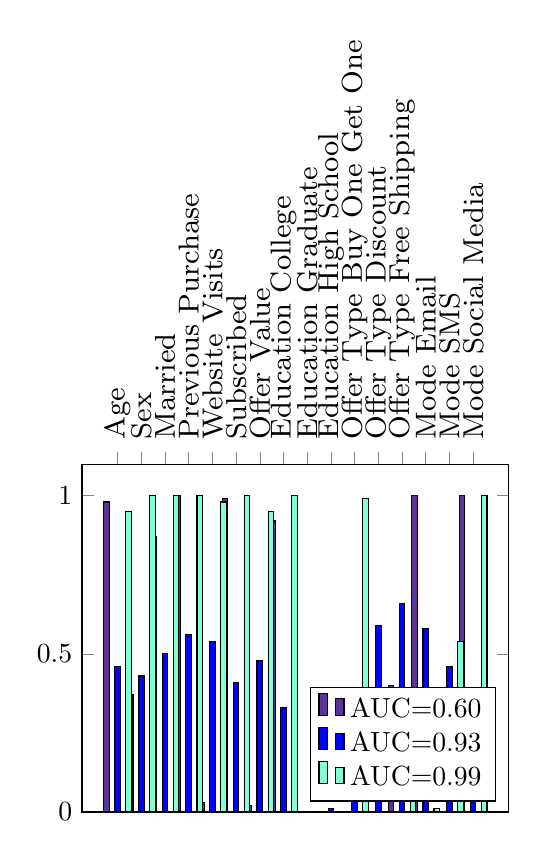
\begin{tikzpicture}
    \begin{axis}[
        ybar,
        ymin=0,
        width  = 7cm,
        height = 6cm,
        bar width=2pt,
        %ylabel={Accuracy},
        %nodes near coords,
        xtick = data,
        table/header=false,
        table/row sep=\\,
        xticklabels from table={\footnotesize
           {Age}\\\footnotesize {Sex}\\\footnotesize {Married}\\\footnotesize {Previous Purchase}\\\footnotesize {Website Visits}\\\footnotesize {Subscribed}\\\footnotesize {Offer Value}\\\footnotesize {Education College}\\\footnotesize {Education Graduate}\\\footnotesize {Education High School}\\\footnotesize {Offer Type Buy One Get One}\\\footnotesize {Offer Type Discount}\\\footnotesize {Offer Type Free Shipping}\\\footnotesize {Mode Email}\\\footnotesize {Mode SMS}\\\footnotesize {Mode Social Media}\\
          }{[index]0},
        %enlarge y limits={value=0.2,upper},
        legend pos=south east,
         xticklabel style={scale=1.3,rotate=90},
        xlabel style={font=\Huge},
        xtick pos=upper,
        xticklabel pos=upper
    ]
     \legend{AUC=0.60, AUC=0.93, AUC=0.99}
    \addplot[fill=RoyalPurple] table[x expr=\coordindex,y index=0]{0.98\\0.37\\0.87\\1.0\\0.03\\0.99\\0.02\\0.92\\0.0\\0.0\\0.0\\0.0\\0.4\\1.0\\0.0\\1.0\\};
    \addplot[fill=blue] table[x expr=\coordindex,y index=0]{0.46\\0.43\\0.5\\0.56\\0.54\\0.41\\0.48\\0.33\\0.0\\0.01\\0.38\\0.59\\0.66\\0.58\\0.46\\0.35\\};
    \addplot[fill=Aquamarine] table[x expr=\coordindex,y index=0]{0.95\\1.0\\1.0\\1.0\\0.98\\1.0\\0.95\\1.0\\0.0\\0.0\\0.99\\0.0\\0.05\\0.01\\0.54\\1.0\\};
    %\pgfplotsinvokeforeach{0,3,4,7,8,11}{\coordinate(l#1)at(axis cs:#1,0);}
    \end{axis}
    \coordinate(bbs)at(current bounding box.south);
    %\foreach[count=\i,evaluate={\s=int(4*\i-1)},evaluate={\e=int(4*(\i-1))}] \text in {Axial,Coronial,Sagittarial}
      %\draw[decorate,decoration=brace]([xshift=8pt]l\s|-bbs)--node[below=5pt]{\text}([xshift=-8pt]l\e|-bbs);
\end{tikzpicture}

              \caption{Spearman rank correlations of ranked feature importance magnitudes from LIME and SHAP against the true ranked magnitudes from $\mathcal{G}$.}
               \label{fig:lime_shap_Spearman_magnitude}
            \end{subfigure}%

            
            \begin{subfigure}{.3\textwidth}
              \centering
               \captionsetup{justification=centering}
              %\includegraphics[width=.9\linewidth]{Figures/lime_shap_Spearman_signed.png}
\pgfplotsset{compat=newest,
		    %every tick label/.append style={rotate=45},
		%xticklabel style={
		%	rotate = 45
		%},
overwrite option/.style args={#1 with #2}{#1=#2,#1/.code=},
		    width=7cm, height=6.15cm,
		    %scale only axis=true,
		    %[...]
                    %axis equal=true,
                    %overwrite option=ymin with -1,
                    %overwrite option=ymax with 1,
		yticklabel style={
			/pgf/number format/fixed,
			/pgf/number format/precision=2
		},
		scaled y ticks=false,
every axis/.append style={
                    %axis x line=middle,    % put the x axis in the middle
                    %axis y line=middle,    % put the y axis in the middle
                    %axis line style={<->}, % arrows on the axis
                    %xlabel={$x$},          % default put x on x-axis
                    %%ylabel={$y$},          % default put y on y-axis
                    label style={font=\large},
                    tick label style={font=\large}  
                    }
}
                            \begin{tikzpicture}
                    \violinsetoptions[
                        averages,
                        data points,
                        scaled,
                    ]{
                        xmin=0,xmax=4,
                        ymin=-.6,ymax=1,
                        % xlabel style={
                        %     yshift = {-2*height("a")}
                        % },
        %ylabel style={
        %    at={(rel axis cs:-0.1,0.5)}
        %},
                        ymajorgrids=true,
                        %ylabel={Spearman Correlation},
                        xlabel={AUC},
                        xlabel style={at={(0,-.08)},below left,yshift=10pt}
                    }
                    \violinplot[%
                    index={SHAP AUC=0.6},
                    relative position=1,
                    color=RoyalPurple,
                    label={0.60},
                    col sep=comma,
                    bandwidth=.05
                    ]{sec4_4_mlp_auc_final.csv}
                    \violinplot[%
                    index={SHAP AUC=0.9},
                    relative position=2,
                    color=blue,
                    label={0.93},
                    col sep=comma,
                    bandwidth=.05
                    ]{sec4_4_mlp_auc_final.csv}
                    \violinplot[%
                    index={SHAP AUC=0.10},
                    relative position=3,
                    color=Aquamarine,
                    label={0.99},
                    bandwidth=.05,
                    col sep=comma,
                    ]{sec4_4_mlp_auc_final.csv}
                \end{tikzpicture}
              \caption{Spearman rank correlations of signed feature importance magnitudes from LIME and SHAP against the true ranking from $\mathcal{G}$.}
               \label{fig:shapcorr}
            \end{subfigure}

            \begin{subfigure}{.3\textwidth}
\pgfplotsset{compat=newest,
		    %every tick label/.append style={rotate=45},
		%xticklabel style={
		%	rotate = 45
		%},
overwrite option/.style args={#1 with #2}{#1=#2,#1/.code=},
		    width=7cm, height=6cm,
		    %scale only axis=true,
		    %[...]
                    %axis equal=true,
                    %overwrite option=ymin with -1,
                    %overwrite option=ymax with 1,
		yticklabel style={
			/pgf/number format/fixed,
			/pgf/number format/precision=2
		},
		scaled y ticks=false,
every axis/.append style={
                    %axis x line=middle,    % put the x axis in the middle
                    %axis y line=middle,    % put the y axis in the middle
                    %axis line style={<->}, % arrows on the axis
                    %xlabel={$x$},          % default put x on x-axis
                    %%ylabel={$y$},          % default put y on y-axis
                    label style={font=\large},
                    tick label style={font=\large}  
                    }
}
            
              \centering
               \captionsetup{justification=centering}
              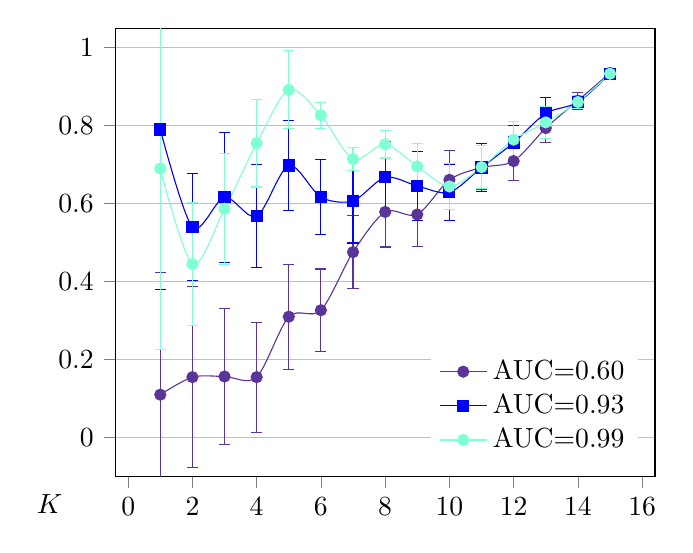
\begin{tikzpicture}
            \begin{axis}[ymin=-.1, ymax=1.05, 
              %ytick={0,1},
              ytick align=outside, ytick pos=left,
              %xtick={0,2,...,10}, 
              xtick align=outside, xtick pos=left,
              ymajorgrids=true,
              xlabel=$K$,
              %ylabel={Recall},
        %ylabel style={
        %    at={(rel axis cs:-0.1,0.5)}
        %},
              legend pos=south east,
              legend style={draw=none},
              xlabel style={at={(-.08,-.08)},below left,yshift=10pt}
              ]

            \addplot+[
              RoyalPurple, mark options={RoyalPurple},
              smooth, 
              error bars/.cd, 
                y fixed,
                y dir=both, 
                y explicit
            ] table [x=K, y=Recall,y error=Error, col sep=comma] {
                K,  Recall,       Error
1, 0.11, 0.31446603773522014
2, 0.155, 0.23241159935586583
3, 0.15666666666666665, 0.17378728435078386
4, 0.155, 0.14115325863841197
5, 0.30999999999999994, 0.13446489534747752
6, 0.32666666666666666, 0.1057281948131679
7, 0.47571428571428565, 0.09317019048477956
8, 0.57875, 0.08998982826919491
9, 0.5722222222222223, 0.08110565299963572
10, 0.6609999999999999, 0.0764027076573451
11, 0.6927272727272731, 0.05599542037014503
12, 0.7091666666666667, 0.04954195356199126
13, 0.7938461538461539, 0.03768445758127965
14, 0.8642857142857144, 0.021536524612697422
15, 0.9353333333333336, 0.01142977386651768
            };
            \addlegendentry{AUC=0.60}
            \addplot+[
              blue, mark options={blue, scale=1.0},
              smooth, 
              error bars/.cd, 
                y fixed,
                y dir=both, 
                y explicit
            ] table [x=K, y=Recall,y error=Error, col sep=comma] {
                    K,  Recall,       Error
1, 0.79, 0.40936018074033237
2, 0.54, 0.13632996217214538
3, 0.6166666666666666, 0.16666666666666663
4, 0.5675, 0.13226370200734164
5, 0.6979999999999998, 0.11545255704960777
6, 0.6166666666666667, 0.09622504486493762
7, 0.607142857142857, 0.1081601536679566
8, 0.6675, 0.09269396807328789
9, 0.6455555555555554, 0.08890993016954553
10, 0.629, 0.07148497051899098
11, 0.6927272727272731, 0.061671083021205594
12, 0.7566666666666667, 0.04380858271151808
13, 0.8315384615384616, 0.04046085599502435
14, 0.8600000000000001, 0.014067598969066614
15, 0.9333333333333336, 2.2316322462394835e-16
            };
            \addlegendentry{AUC=0.93}
            \addplot+[
              Aquamarine, mark options={Aquamarine, scale=1.0},
              smooth, 
              error bars/.cd, 
                y fixed,
                y dir=both, 
                y explicit
            ] table [x=K, y=Recall,y error=Error, col sep=comma] {
                    K,  Recall,       Error
1, 0.69, 0.4648231987117317
2, 0.445, 0.15723301886761007
3, 0.5866666666666667, 0.14307823199697595
4, 0.755, 0.11225422086055427
5, 0.892, 0.1001816531924066
6, 0.8266666666666665, 0.03282439759448874
7, 0.714285714285714, 0.0287153661502632
8, 0.7525, 0.0354445077736048
9, 0.6955555555555556, 0.05828320758006698
10, 0.644, 0.05915226030330453
11, 0.693636363636364, 0.05580875600520632
12, 0.7641666666666667, 0.04595751466038848
13, 0.8084615384615387, 0.04162585413792407
14, 0.8607142857142859, 0.015645922396970754
15, 0.9333333333333336, 2.2316322462394835e-16
            };
            \addlegendentry{AUC=0.99}
            \end{axis}
            \end{tikzpicture}

              \caption{Spearman rank correlations of signed feature importance magnitudes from LIME and SHAP against the true ranking from $\mathcal{G}$.}
               \label{fig:lime_shap_Spearman_signed}
            \end{subfigure}


            
            %\caption{violin plots of Spearman correlations between LIME and SHAP feature importance rankings, both signed and unsigned, against the true rankings. }
           %\label{fig:lime_shap_Spearman_signed_mag}
        \end{figure}
	
\end{document}
